% Research paper for the DWM practical - IEEE conference format (IEEEtran).
% Same content as the WDL paper plus the data warehouse, rewritten in new wording.
% Build: tectonic paper_dwm.tex. Numbers: reports/final and data/warehouse.db.
\documentclass[conference]{IEEEtran}
\usepackage[T1]{fontenc}
\usepackage{cite}
\usepackage{amsmath}
\usepackage{newtxtext,newtxmath}
\usepackage{graphicx}
\usepackage{booktabs}
\usepackage{multirow}
\usepackage{xcolor}
\usepackage{tikz}
\usetikzlibrary{arrows.meta,positioning,fit}
\usepackage{url}
\usepackage[hidelinks]{hyperref}

\setlength{\textfloatsep}{8pt plus 2pt minus 2pt}
\setlength{\dbltextfloatsep}{8pt plus 2pt minus 2pt}
\setlength{\floatsep}{6pt plus 2pt minus 2pt}
\setlength{\dblfloatsep}{6pt plus 2pt minus 2pt}
\setlength{\abovecaptionskip}{3pt}

\renewcommand{\IEEEbibitemsep}{0pt plus .5pt}
\begin{document}

\title{Sentinel: A CNN-LSTM Intrusion Detector that Defers Uncertain Flows to Analysts, with Gated Retraining and an OLAP Data Warehouse}

\author{
\IEEEauthorblockN{Jai Chavan, Jeet Mane, Amaan Khan}
\IEEEauthorblockA{Department of Computer Engineering\\
Vidyalankar Institute of Technology, Mumbai, India\\
jai.chavan@vit.edu.in, jeet.mane@vit.edu.in, amaan.khan@vit.edu.in}
\and
\IEEEauthorblockN{Dr. Kavita Shirsat}
\IEEEauthorblockA{Department of Computer Engineering\\
Vidyalankar Institute of Technology, Mumbai, India}
}

\maketitle

\begin{abstract}
High scores on a fixed benchmark tell little about how a learned intrusion detector behaves when
real traffic stops resembling its training data. Sentinel is a prototype designed around that
problem. A convolutional network followed by an LSTM (CNN-LSTM) labels every network flow, and a
second stage decides whether the label can be trusted or whether a security analyst must look at
the flow first. That decision uses three signals: the entropy of the temperature-scaled output, a
Mahalanobis distance in the network's 128-value hidden representation, and the voting behaviour of
a Random Forest that serves as an independent opinion. Analysts record a verdict together with the
reason and the evidence behind it; these records become searchable cases, and they reach the model
only after an administrator verifies them and a retrained version passes limits that were fixed
before any retraining. The system was evaluated on the corrected CIC-IDS2017 release after
identifier fields were removed and 385,106 repeated flows were merged prior to splitting. Of
257,222 test flows, 1.48\% were referred to the analyst; this small set contained 98.9\% of the
network's misclassifications, the flows decided without a person were 99.999\% correct, only two
attack flows were closed as benign, and no benign flow was raised as an alert. When each attack
family was left out of training in turn, the network on its own let up to 97\% of the unseen
attack pass silently, while the full rule held this to at most 10.2\% for five of six families; SSH
password guessing was never caught. Finally, an extract-transform-load (ETL) process copies all
1,714,812 flows, together with the platform's alerts and reviews, into a dimensional data warehouse
that supports OLAP analysis and has no influence on detection.
\end{abstract}

\begin{IEEEkeywords}
intrusion detection, CNN-LSTM, uncertainty, human-in-the-loop, novel attacks, CIC-IDS2017, data warehouse, ETL, OLAP
\end{IEEEkeywords}

%=====================================================================
\section{Introduction}
An early experiment in this project set the direction for the rest of it. A Random Forest that
trained in a few minutes reached 99.97\% accuracy on a random split of CIC-IDS2017. When a basic
model gets that close to perfect, the same number cannot tell a useful detector apart from a
fragile one. Such figures are inflated in three ways. Public flow datasets contain wrong labels and
repeated rows that end up on both sides of the train-test boundary
\cite{engelen2021troubleshooting,liu2022error}. Fields that identify machines or sessions allow a
model to memorise instead of generalise \cite{arp2022dos}. Most importantly, a detector in service
will eventually meet an attack it was never trained on, and the softmax output gives no dependable
warning when this happens \cite{sommer2010outside,hendrycks2017baseline}.

The starting point is the uncertainty-aware adaptive IDS of de Nascimento and Hou
\cite{refpaper2025}, which combines a CNN-LSTM, cWGAN-GP oversampling and analyst feedback and
reports an F1 of 94.3\%, precision of 92.1\%, detection rate of 96.6\% and binary accuracy of
98\%. That classifier was re-implemented and the concept was developed into a working application. The guiding
question is therefore not how accurate the network is, but which flows it may settle by itself and
which ones need a human decision first.

Three contributions follow.
\begin{enumerate}
\item On the corrected CIC-IDS2017 data, with shortcut fields removed, duplicates merged before
splitting and three random seeds, the CNN-LSTM is compared against Random Forest and LightGBM, and
ablations test the effect of the LSTM layer and of synthetic minority samples.
\item Experiments that hold out whole attack families, or whole capture days, show that the
network's own uncertainty misses most new attacks; a combined rule using entropy, embedding
distance and a tree-ensemble opinion is proposed, which hands the majority of them to a person.
\item The entire loop is built as software: traffic replay, an analyst screen that records why a
verdict was given, a case store with similarity search, and retraining that requires pre-set
limits and administrator approval and supports live deployment and rollback.
\end{enumerate}
A dimensional data warehouse, loaded by full and incremental ETL, additionally lets the traffic
history, the alerts and the analyst decisions be explored with OLAP operations.

%=====================================================================
\section{Related Work}
Five bodies of work inform the design: the benchmark and its documented problems, classifiers for
tabular flow data, methods that estimate when a prediction should not be trusted, generative
oversampling, and data warehousing. Table~\ref{tab:related} lists, for each source, the idea that
was borrowed and how Sentinel applies or changes it.

\begin{table*}[t]
\caption{Earlier work and its role in Sentinel}
\label{tab:related}
\centering
\scriptsize
\begin{tabular}{p{1.6cm}p{6.9cm}p{8.35cm}}
\toprule
Source & Key idea & Use in Sentinel \\
\midrule
\cite{sharafaldin2018toward} & Labelled flows from five capture days (CIC-IDS2017) & The only data used for training and testing \\
\cite{engelen2021troubleshooting,liu2022error} & Errors in flows and labels identified and fixed in a new release & The fixed files are used, and repeated rows are merged before splitting \\
\cite{arp2022dos} & Leakage, shortcut features and weak baselines mislead security ML & Host and port fields removed; tree models trained on the same inputs \\
\cite{sommer2010outside} & Real networks keep producing unseen activity & Reason for leaving whole attack families out of training \\
\cite{refpaper2025} & CNN-LSTM with cWGAN-GP and analyst feedback & Network re-implemented; feedback made verified, gated and reversible \\
\cite{hochreiter1997lstm} & Recurrent memory with gates & LSTM placed after the convolution layers \\
\cite{breiman2001random,ke2017lightgbm} & Bagging and boosting of decision trees & Baselines; the forest also gives the second opinion \\
\cite{guo2017calibration} & Rescaling logits with a single temperature & Fitted on one half of the validation data \\
\cite{hendrycks2017baseline} & Low softmax confidence often marks errors & Entropy is one of the routing signals \\
\cite{lee2018simple} & Distance from class centres reveals unfamiliar inputs & Computed on the LSTM hidden vector \\
\cite{lakshminarayanan2017simple} & Separately trained models disagree on unfamiliar inputs & Network-forest disagreement sends a flow to review \\
\cite{geifman2017selective} & Balancing how often to abstain against error on the rest & Review rate versus error on automatically handled flows \\
\cite{mirza2014conditional,gulrajani2017improved} & Conditional GAN trained with gradient penalty & Synthetic minority rows in an ablation \\
\cite{chaudhuri1997overview,kimball2013toolkit} & Warehouse design, dimensional models and OLAP & Star, snowflake and constellation schemas for flows, alerts and reviews \\
\bottomrule
\end{tabular}
\end{table*}

%=====================================================================
\section{Data Preparation}
The experiments rely on the corrected CIC-IDS2017 release \cite{engelen2021troubleshooting,liu2022error},
which provides one file for each weekday from Monday to Friday. In total there are 2,099,976
records, 91 columns and 27 different label values. A checking script found no blank cells and just
five records with infinite rate values. As stored, no two rows were the same, but after the
identifying fields were put aside every eighth row (12.5\%) was a copy of another.

\textit{Fields excluded.} Identifiers such as the flow ID, both addresses, the sending port, the time of capture
and the row index say which machines communicated rather than how they behaved, so the classifier never
receives them. The corrected files also contain an ``Attempted Category'' field that is set only for
attack rows; because it gives away the label, it is removed too. The destination port is dropped as
well, since in this capture port 21 almost always means FTP-Patator, a link that a model could use
without understanding the attack.

\textit{Class grouping.} Unsuccessful (``Attempted'') attacks are merged into the attack they
belong to. \textit{Infiltration--Portscan} becomes \textit{Portscan}, because the two cannot be told
apart from the features, and the brute-force, XSS and SQL-injection web attacks are combined into a
single Web Attack class. This gives 13 classes. The two smallest classes, Heartbleed with 11 rows and Infiltration
with 81, remain in the data but are marked: their scores depend on very few test flows, so a
``reliable'' macro-F1 that leaves them out is reported alongside the full one.

\textit{Merging repeats before splitting.} Rows with the same input features and the same label are
kept only once, which deletes 385,106 rows; another 58 rows whose identical features appear with
two labels are discarded, since no model could separate them. Once the destination port was gone,
scan traffic proved extremely repetitive, with Portscan falling from 230,833 to 7,695 unique flows.
The resulting 1,714,812 flows are split 70/15/15 with stratification by class
(Table~\ref{tab:classes}); hashing each feature vector shows that no flow appears in two partitions.

\textit{Feature processing.} All statistics in this step come from the training partition only.
Missing and infinite entries are replaced with the training median. Byte counts and durations cover
many orders of magnitude, so every value is transformed as $\mathrm{sign}(x)\log(1+|x|)$. A constant
column and 17 columns that are nearly copies of another ($|\rho|>0.99$) are removed, which leaves 64
inputs that are then standardised. The fitted transform is stored with each model, along with the
column order and the class list, so that the web application processes flows exactly as in training.

\begin{table}[t]
\caption{Number of flows per class after grouping and merging repeats}
\label{tab:classes}
\centering
\footnotesize
\begin{tabular}{lrrr}
\toprule
Class & Test & Validation & Train \\
\midrule
Normal (BENIGN) & 213,516 & 213,517 & 996,410 \\
Botnet & 288 & 288 & 1,343 \\
DDoS & 14,271 & 14,272 & 66,601 \\
DoS GoldenEye & 1,147 & 1,147 & 5,353 \\
DoS Hulk & 23,858 & 23,857 & 111,333 \\
DoS Slowhttptest & 766 & 766 & 3,576 \\
DoS Slowloris & 856 & 855 & 3,992 \\
FTP-Patator & 598 & 597 & 2,789 \\
Heartbleed$^\dagger$ & 1 & 2 & 8 \\
Infiltration$^\dagger$ & 10 & 10 & 46 \\
Portscan & 1,155 & 1,154 & 5,386 \\
SSH-Patator & 448 & 448 & 2,092 \\
Web Attack & 308 & 309 & 1,439 \\
\midrule
All classes & 257,222 & 257,222 & 1,200,368 \\
\bottomrule
\multicolumn{4}{l}{$^\dagger$Too few flows for dependable per-class scores.}
\end{tabular}
\end{table}

%=====================================================================
\section{Proposed Method}

\begin{figure*}[t]
\centering
\resizebox{0.8\textwidth}{!}{%
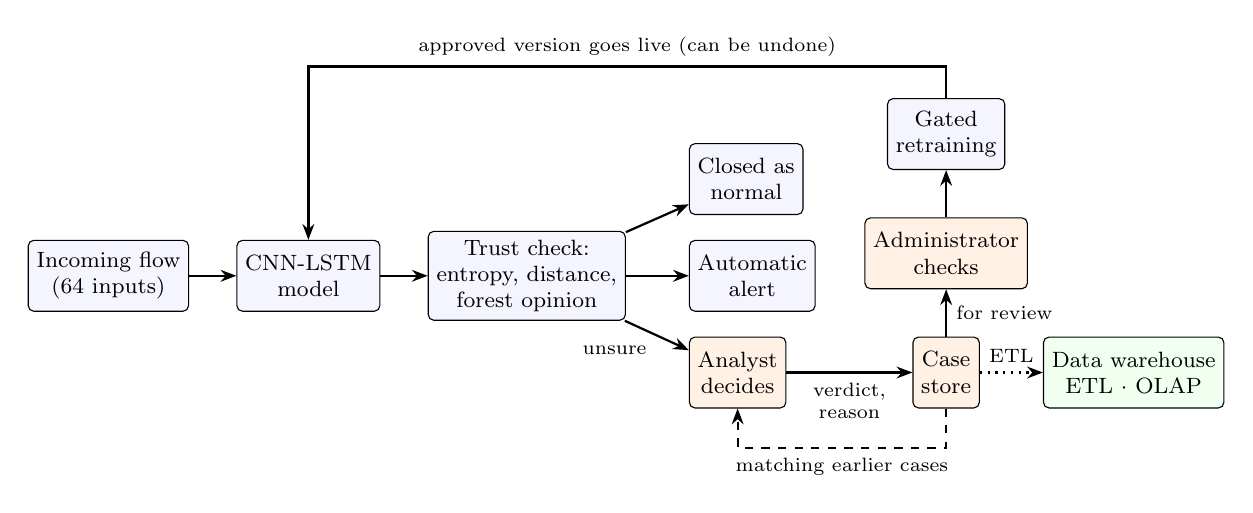
\begin{tikzpicture}[
  box/.style={draw, rounded corners=2pt, align=center, font=\footnotesize, minimum height=9mm, inner sep=3pt, fill=blue!4},
  hum/.style={box, fill=orange!10},
  arr/.style={-{Stealth[length=2mm]}, thick},
  lab/.style={font=\scriptsize, align=center}]
\node[box] (flow) {Incoming flow\\(64 inputs)};
\node[box, right=6mm of flow] (cnn) {CNN-LSTM\\model};
\node[box, right=6mm of cnn] (unc) {Trust check:\\entropy, distance,\\forest opinion};
\node[box, above right=2mm and 8mm of unc] (benign) {Closed as\\normal};
\node[box, right=8mm of unc] (alert) {Automatic\\alert};
\node[hum, below right=2mm and 8mm of unc] (analyst) {Analyst\\decides};
\node[hum, right=16mm of analyst] (kr) {Case\\store};
\node[hum, above=6mm of kr] (admin) {Administrator\\checks};
\node[box, above=6mm of admin] (retrain) {Gated\\retraining};
\draw[arr] (flow) -- (cnn);
\draw[arr] (cnn) -- (unc);
\draw[arr] (unc) -- (benign);
\draw[arr] (unc) -- (alert);
\draw[arr] (unc) -- node[lab, below left]{unsure} (analyst);
\draw[arr] (analyst) -- node[lab, below]{verdict,\\reason} (kr);
\draw[arr] (kr) -- node[lab, right]{for review} (admin);
\draw[arr] (admin) -- (retrain);
\draw[arr] (retrain.north) |- ++(0,4mm) -| node[lab, above, pos=0.25]{approved version goes live (can be undone)} (cnn.north);
\draw[arr, dashed] (kr.south) |- ++(0,-5mm) -| node[lab, below, pos=0.25]{matching earlier cases} (analyst.south);
\node[box, right=8mm of kr, fill=green!6] (dw) {Data warehouse\\ETL $\cdot$ OLAP};
\draw[arr, dotted] (kr) -- node[lab, above]{ETL} (dw);
\end{tikzpicture}}
\caption{Architecture of Sentinel. Flows reach the analyst only when the router is unsure; verified
decisions change the model only through approved retraining; the data warehouse, loaded by ETL,
serves analysis alone.}
\label{fig:system}
\end{figure*}

\subsection{Network architecture and training}
The layers follow Table 5 of \cite{refpaper2025}, adapted to 64 inputs instead of 46. The
standardised vector is treated as a one-channel sequence of length 64. It passes a convolution with
64 filters (kernel 5, ReLU), max-pooling by a factor of two, a convolution with 128 filters (kernel
3, ReLU), a 128-unit LSTM, 30\% dropout and a linear layer with 13 outputs. The final LSTM state
$\mathbf{z}\in\mathbb{R}^{128}$ is used as the flow's embedding, because the routing stage measures
distances there. The network is trained with plain cross-entropy and AdamW (learning rate
$10^{-3}$, batch size 1,024, cosine schedule) for at most 20 epochs, keeping the epoch with the
highest validation macro-F1. A class-weighted loss was not used because it would distort the
probabilities that routing depends on. In the first runs, however, Heartbleed and Infiltration were
never predicted and validation macro-F1 stayed around 0.85. Duplicating the training rows of every
class with fewer than 1,000 examples up to that number (on the training partition only) solved this.

\subsection{Baselines and ablations}
A Random Forest of 100 trees and a LightGBM model are trained on the identical 64 transformed
inputs. LightGBM uses early stopping on validation loss; its first run diverged after 12 rounds,
which was cured by limiting leaf output values. Three ablations examine the design: the LSTM is
replaced by global average pooling, GAN-generated minority rows are added, and temperature scaling
is skipped.

\subsection{Synthetic minority samples}
The augmentation ablation uses a Wasserstein GAN that is conditioned on the class and
regularised by a gradient penalty \cite{mirza2014conditional,gulrajani2017improved}. Both generator and critic have two hidden layers
of 256 units, the penalty weight is 10, and the critic takes five steps for every generator step.
Only classes holding between 100 and 5,000 training rows are filled, each up to 5,000 rows, and a
synthetic row is kept only if the baseline forest assigns it to its intended class. Whereas the
reference work seeds the generator from a VAE, Gaussian noise is used here.

\subsection{Calibration and uncertainty scores}
The validation partition is divided into two stratified halves: a calibration half, on which all
parameters in this subsection are fitted, and an evaluation half, kept for judging them. One
temperature $T$ \cite{guo2017calibration} rescales the logits, and each flow is then given two
scores:
\begin{equation}
H(\mathbf{x}) = -\frac{1}{\log K}\sum_{k=1}^{K} p_k \log p_k, \quad
\mathbf{p} = \mathrm{softmax}(\mathbf{f}(\mathbf{x})/T),
\end{equation}
the entropy over the $K=13$ classes normalised to the range 0 to 1, and the squared Mahalanobis
distance between the embedding and the closest class centre \cite{lee2018simple}
\begin{equation}
D(\mathbf{x}) = \min_{c} (\mathbf{z}-\boldsymbol{\mu}_c)^\top \boldsymbol{\Sigma}^{-1} (\mathbf{z}-\boldsymbol{\mu}_c),
\end{equation}
with class centres $\boldsymbol{\mu}_c$ and a shared covariance $\boldsymbol{\Sigma}$ (plus a small
ridge for numerical stability) estimated from training embeddings. Entropy reflects indecision
among known classes, while distance reflects flows that look like no known class. Both thresholds
are taken from the calibration half: $\tau_H$ is exceeded by the 1\% least certain flows and $\tau_D$
by the 0.5\% most distant ones.

\subsection{Combined routing rule}
A flow counts as \emph{uncertain} when
\begin{equation}
H>\tau_H \;\lor\; D>\tau_D \;\lor\; u_{\mathrm{RF}}>\tau_{\mathrm{RF}} \;\lor\; \hat{y}_{\mathrm{RF}}\neq\hat{y},
\end{equation}
and it is then assigned one of three outcomes:
\begin{equation}
\text{decision}(\mathbf{x}) =
\begin{cases}
\text{review} & \text{if uncertain},\\
\text{auto-alert} & \text{else if } \hat{y}\neq\text{BENIGN},\\
\text{auto-benign} & \text{otherwise,}
\end{cases}
\end{equation}
where $\hat{y}$ and $\hat{y}_{\mathrm{RF}}$ are the classes predicted by the CNN-LSTM and the
Random Forest. The forest's doubt $u_{\mathrm{RF}} = 1-\max_k p^{\mathrm{RF}}_k$ is the share of
trees that voted for some other class, and $\tau_{\mathrm{RF}}$ marks the 0.5\% most
doubtful calibration flows. In plain terms, a flow skips the analyst only if three things hold at
once: the network is clear about its answer, the flow looks like familiar traffic, and an
independently built forest is sure and agrees. The two
forest conditions were added after the held-out-family experiment (Section~\ref{sec:loao}) revealed
how often the network alone ignored new attacks, so that experiment does not independently support
the rule; the test partition, used once after the rule was fixed, does.

\subsection{Analyst platform}
Fig.~\ref{fig:system} shows how the components are connected. A FastAPI service with SQLite storage
forms the back end, and a React front end offers four sections: a public About page, the analyst
console, the administration console and a data-warehouse view (Section~\ref{sec:dw}).
\begin{itemize}
\item \textit{Replay.} A background task sends the unused test flows to the current model in batches
of adjustable size to imitate live traffic. The true label of each record is stored only so the
administrator can track live accuracy; it is never given to the model or shown to analysts, which
an automated test verifies.
\item \textit{Analyst console.} A referred flow opens on a single screen showing where and when
the flow happened, the top three candidate classes, what the forest predicted, both uncertainty scores against
their thresholds, the six most unusual features compared with training data, and
closely matching past cases. The analyst answers malicious, benign or unsure, picks a class, a
written reason, context and evidence, a confidence level and optional tags.
\item \textit{Case store.} Every reply is stored as a searchable case. Cases are compared by the
cosine similarity of their CNN-LSTM embeddings, and because a retrained network places flows in a
different space, stored embeddings are recalculated each time a new model is put into use.
\item \textit{Gated retraining.} Feedback becomes usable for training only after an administrator
marks it verified. Verified items are split 70/30. The current network is fine-tuned on the 70\%
plus 200,000 rows sampled from the original training data, so that older attack families are not
forgotten, and is then recalibrated. Old and new versions are compared on two fixed benchmarks: the
evaluation half of the validation data and the 30\% of feedback held back. The acceptance limits
live in a configuration file and are copied into each job when it starts: reliable macro-F1 may
drop by up to 0.5 points, false positives may increase by up to 0.05 points, and accuracy
on held-back feedback must not decrease. A candidate that passes still needs administrator
approval; deployment and rollback swap the model in memory without stopping the service, and every
step is written to an audit log.
\end{itemize}

\subsection{Data warehouse for analysis}\label{sec:dw}
The operational (OLTP) database is designed for many small writes, not for questions that span the
whole history. A separate, read-only data warehouse was therefore built in its own SQLite file
\cite{chaudhuri1997overview,kimball2013toolkit}. It is used for analysis only and never affects
training, tuning, prediction or analyst decisions.
\begin{itemize}
\item \textit{Schemas.} The fact table \texttt{fact\_flow} stores one row for each of the 1,714,812
flows, with packet, byte and duration measures and keys to five hierarchical dimensions: time (day,
part of day, hour, minute), attack (benign or malicious, category, class), service (port range,
service, port), protocol and data partition, forming a star schema. A snowflake version places the
attack category and the calendar date in separate tables. A fact constellation connects an alert
fact table (prediction, confidence, entropy, distance, route) and a factless review table (analyst
decisions) through shared time, attack and model dimensions. An hourly aggregate of 606 rows and
two data marts bring the total to 22 tables.
\item \textit{ETL.} \emph{Extract} reads the cleaned partitions, the raw capture files for
timestamps, and the platform database through a read-only connection. \emph{Transform} links each
flow to its raw record (all 1,714,812 linked), replaces missing or negative measures with zero,
turns timestamps into minute keys, maps ports to services and classes to categories, and assigns
surrogate keys. \emph{Load} writes the warehouse to a staging file and then replaces the old one in a
single step (full load, about 25\,s). An incremental load adds only alerts beyond a stored watermark
(about 0.3\,s when there is nothing new) and performs a clean reload if the platform database was reset.
\item \textit{OLAP.} A cube view supports roll-up, drill-down, slice, dice and pivot along these
hierarchies and displays the result as a table, a chart and a three-dimensional cube. Each action
is turned into a parameterised SQL query, and questions that need time no finer than the hour are
answered from the aggregate table rather than the full fact table.
\end{itemize}

%=====================================================================
\section{Evaluation Protocol}
All models are trained on the training partition, and every setting or design choice was made
using validation results alone. The test partition was opened once, after the routing rule and all
parameters had been fixed. Every model was trained with seeds 42, 7 and 2025, and the tables report
the mean and standard deviation; the deployed application runs the network and forest from seed 42. ``Accuracy''
treats a prediction as right only when the exact class out of 13 is correct, whereas the remaining
measures (precision, recall or detection rate, F1, FPR and FNR) count every attack type as one
positive class, following the reference work. The hardware was a single laptop (Intel Core
i5-1240P processor, 7.7\,GB memory, 4\,GB NVIDIA RTX 2050 GPU), and the software used PyTorch \cite{paszke2019pytorch} and
scikit-learn \cite{pedregosa2011scikit}.

\textit{Generalisation experiments.} Two additional tests use training and validation rows only.
(i) \emph{Held-out family:} for each of six attacks, all rows of that attack are removed from the
training and calibration data, everything is fitted again with a single seed (the CNN-LSTM for eight
epochs, then temperature, thresholds and forest), and the router's treatment of that attack is recorded.
(ii) \emph{Day split:} models are trained on Monday to Wednesday and tested on Thursday and Friday,
whose attack types do not appear earlier in the week.

%=====================================================================
\section{Results}

\subsection{Test-set classification}
Table~\ref{tab:main} lists each model with the published numbers of the reference design in the
first row. All five trained models, including the re-implemented CNN-LSTM, exceed those figures on every
binary measure. This should not be taken as an advance over that work, since the data release, the
handling of repeats and the removed fields all differ, and such choices are known to shift results
considerably \cite{engelen2021troubleshooting,arp2022dos}. Among the models trained here, the tree
ensembles lead. On the reliable classes the forest's macro-F1 is 99.23\%, against 98.09\% for the
CNN-LSTM, and its false-alarm rate is roughly three times lower (0.020\% versus 0.059\%).

\begin{table*}[t]
\caption{Results on the 257,222 test flows: mean $\pm$ standard deviation over three seeds (\%)}
\label{tab:main}
\centering
\scriptsize
\setlength{\tabcolsep}{3pt}
\begin{tabular}{lccccccc}
\toprule
Model & F1 & Precision & Det. rate & Acc. (13-cl.) & M-F1 (rel.) & M-F1 (all) & FPR \\
\midrule
Published reference \cite{refpaper2025} & 94.3 & 92.1 & 96.6 & 98.0$^\ast$ & -- & -- & -- \\
Random Forest & \textbf{99.91} $\pm$ 0.00 & \textbf{99.90} $\pm$ 0.00 & \textbf{99.92} $\pm$ 0.00 & \textbf{99.97} $\pm$ 0.00 & \textbf{99.23} $\pm$ 0.02 & \textbf{99.07} $\pm$ 0.22 & \textbf{0.020} $\pm$ 0.000 \\
LightGBM & 99.88 $\pm$ 0.01 & 99.84 $\pm$ 0.01 & 99.91 $\pm$ 0.01 & 99.96 $\pm$ 0.00 & 99.03 $\pm$ 0.05 & 98.32 $\pm$ 0.04 & 0.033 $\pm$ 0.003 \\
CNN-LSTM & 99.73 $\pm$ 0.16 & 99.71 $\pm$ 0.07 & 99.75 $\pm$ 0.24 & 99.89 $\pm$ 0.07 & 98.09 $\pm$ 0.99 & 96.71 $\pm$ 3.06 & 0.059 $\pm$ 0.015 \\
CNN-LSTM with GAN rows & 99.80 $\pm$ 0.04 & 99.74 $\pm$ 0.03 & 99.86 $\pm$ 0.05 & 99.92 $\pm$ 0.02 & 98.47 $\pm$ 0.25 & 97.46 $\pm$ 1.36 & 0.054 $\pm$ 0.005 \\
CNN without LSTM & 99.46 $\pm$ 0.05 & 99.70 $\pm$ 0.01 & 99.23 $\pm$ 0.10 & 99.80 $\pm$ 0.02 & 96.39 $\pm$ 0.32 & 94.12 $\pm$ 1.42 & 0.062 $\pm$ 0.002 \\
\bottomrule
\multicolumn{8}{l}{$^\ast$The reference reports binary accuracy. ``Reliable'' omits Heartbleed and Infiltration. F1, precision, detection rate and FPR treat all attacks as one class.}
\end{tabular}
\end{table*}

\begin{table}[t]
\caption{Recall for each class on the test set (\%, average of three seeds)}
\label{tab:perclass}
\centering
\scriptsize
\begin{tabular}{lccc}
\toprule
Class & CNN-LSTM & Random Forest & LightGBM \\
\midrule
Normal (BENIGN) & 99.94 & 99.98 & 99.97 \\
Botnet & 89.35 & 94.79 & 92.01 \\
DDoS & 99.99 & 100.00 & 100.00 \\
DoS GoldenEye & 98.23 & 100.00 & 99.91 \\
DoS Hulk & 99.90 & 100.00 & 99.99 \\
DoS Slowhttptest & 98.96 & 98.87 & 99.09 \\
DoS Slowloris & 99.10 & 100.00 & 100.00 \\
FTP-Patator & 99.78 & 100.00 & 100.00 \\
Heartbleed$^\dagger$ & 100.00 & 100.00 & 100.00 \\
Infiltration$^\dagger$ & 93.33 & 93.33 & 80.00 \\
Portscan & 96.65 & 99.65 & 99.65 \\
SSH-Patator & 99.48 & 99.70 & 99.70 \\
Web Attack & 96.54 & 97.94 & 98.38 \\
\bottomrule
\multicolumn{4}{l}{$^\dagger$Only 1 and 10 test flows.}
\end{tabular}
\end{table}

Per class (Table~\ref{tab:perclass}), the network falls behind mainly on Portscan, Botnet and Web
Attack. For all three models Botnet is the hardest of the reliable classes, with recall from 89\% to 95\%.

\subsection{Ablation results}
Removing the LSTM lowers reliable macro-F1 by 1.7 points and Portscan recall from 96.7\% to 88.8\%,
which shows that the recurrent layer is worth keeping. Synthetic minority rows raise average
reliable macro-F1 by 0.4 points and make the seeds more consistent (standard deviation down from
0.99 to 0.25), but the improvement is smaller than the variation between seeds. The reason is easy
to see: a classifier trained to separate real from synthetic rows does so perfectly (AUC 1.0) for
all six augmented classes, because real flow features are whole-number counts while the generator
produces continuous values. Temperature scaling chose $T=1.01$, so the network was already
calibrated (calibration error 0.023\% before and 0.022\% after), and leaving this step out makes no
measurable difference.

\subsection{Routing outcome}
Table~\ref{tab:routing} describes the configuration used in the application. About one flow in 68
(1.48\%) goes to an analyst, and this short queue holds 98.9\% of the network's errors. The other
98.5\% of traffic, which no one inspects, is labelled correctly 99.999\% of the time. Only two of the 43,706
attack flows were wrongly closed, and no benign flow became a confident alert. Compared with
routing on the network's two scores alone, adding the forest costs 0.15 percentage points of extra
review and reduces missed attacks from seven to two. Review effort concentrates where the classifier
is weakest: the router refers every Infiltration flow, nearly all Web Attack flows (99.7\%), three quarters of
DoS Slowhttptest, about two thirds of Botnet (63\%) and over a third of Portscan (38\%), against under 1\% for BENIGN, DDoS and DoS Hulk.

\begin{table}[t]
\caption{Routing of the test set by the deployed configuration}
\label{tab:routing}
\centering
\footnotesize
\begin{tabular}{lcc}
\toprule
Measure & Network only & With forest \\
\midrule
Share of flows for review & 1.33\% & 1.48\% \\
Mistakes found in review & 96.0\% & \textbf{98.9\%} \\
Correct labels without review & 99.997\% & \textbf{99.999\%} \\
Attacks closed as normal & 7 & \textbf{2} \\
Normal flows raised as alerts & 0 & 0 \\
\bottomrule
\end{tabular}
\end{table}

\subsection{Held-out attack families}
\label{sec:loao}
Fig.~\ref{fig:loao} shows, for each held-out family, how much of its traffic was closed automatically as normal;
these are the attacks that would have gone unnoticed. The first round of this experiment
is what reshaped the design. Using only its own two scores, the network let through 80.5\% of the
unseen Portscan flows and 32.9\% of the unseen Botnet flows, whereas a Random Forest judged only on
the spread of its tree votes let through 5.3\% and 10.8\%. The network was also unstable between
runs: unseen web attacks were missed 13.1\% of the time in the first round but 97.0\% in the round
shown in the figure. The combined rule gave the lowest miss rate for five of the six families and
stayed at or below 10.2\% for them, at the cost of reviewing about 1.4\% of normal traffic, compared
with 0.55\% for the forest alone. SSH brute force escaped every variant, because each login attempt
on its own is indistinguishable from a legitimate SSH session.

\begin{figure}[t]
\centering
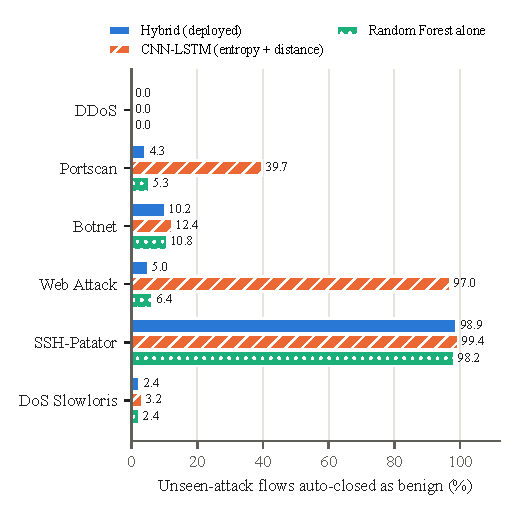
\includegraphics[width=0.56\columnwidth]{figs/loao_missed.pdf}
\caption{Held-out attack families: fraction of each unseen attack's flows closed automatically as
benign (lower is better). The pipeline is retrained without that attack for each group.}
\label{fig:loao}
\end{figure}

\subsection{Held-out days}
If the models only learn from Monday, Tuesday and Wednesday and are then tested on the last two
days, 1.38\% of attack flows slip through the combined rule. Entropy alone would miss 35.28\%, and adding the embedding
distance lowers this to 16.46\%, so the distance score clearly contributes, yet only the forest's
opinion brings the misses close to the forest's own level (1.45\%). The share of normal traffic sent
for review grows to 0.76\%, versus 0.50\% for the forest by itself. Botnet is again the weakest
class, with 37.7\% of its flows closed without review.

\subsection{Platform and warehouse}
During replay the service uses about 0.55\,ms of CPU time per flow, including the forest. An
automated test performs a complete session (replay, analyst verdicts, verification, retraining,
deployment and rollback) and checks that no response sent to analysts includes a true label.

In the warehouse, the query ``flows per attack class per day'' needs about 2.3\,s on the fact table
of 1.7 million rows but only about 0.3\,ms on the hourly aggregate, returning the same result; at
category level the star schema answers in 2,046\,ms and the snowflake in 2,312\,ms, the difference
coming from its additional joins. The OLAP operations also describe the dataset: Monday contains no
attacks, a drill-down places 158,662 of Wednesday's 177,506 denial-of-service flows in one hour, and
a slice on the service dimension shows that 94.4\% of all attack flows used HTTP.

%=====================================================================
\section{Discussion}
\textit{A confident model is not a safe one.} Relying on its own scores, the network allowed as much
as 97\% of a new attack through, and the size of this failure varied between runs. The most
effective remedy was to add a model based on completely different principles and to pass any
disagreement to a person, which agrees with \cite{lakshminarayanan2017simple}.

\textit{Limitations.} Because the classifier judges each flow on its own, it misses attacks that
only stand out when many connections are viewed together (for example SSH password guessing and
some of the botnet flows); this would need features that summarise what a host does over a period
of time.

%=====================================================================
\section{Conclusion}
Sentinel was built to be an intrusion detector that recognises when a decision should go to a
person. With leakage carefully controlled, the CNN-LSTM performs close to strong tree models and
above the published figures of the reference design, but its own uncertainty fails on attacks it
has not seen. Pairing it with a Random Forest repairs most of this: just 1.48\% of traffic requires
a human, almost every network error (98.9\%) falls inside that portion, and most flows of held-out
attack families are seen by an analyst rather than being closed unnoticed. Analyst knowledge returns to the
model only through verified, limit-checked and administrator-approved retraining that can be
reversed, and a separate data warehouse opens the full traffic and decision history to OLAP
analysis. Future work covers features summarising many flows per host, retraining the forest
together with the network, and evaluation on CSE-CIC-IDS2018.

\section*{Acknowledgment}
The authors thank Dr. Kavita Shirsat for her guidance during this project.

%=====================================================================
\begin{thebibliography}{99}

\bibitem{refpaper2025}
C.~M. de~Nascimento and J.~Hou, ``Uncertainty-aware adaptive intrusion detection using hybrid CNN-LSTM with cWGAN-GP augmentation and human-in-the-loop feedback,'' \textit{Safety}, vol.~11, no.~4, Art.~no.~120, Dec. 2025, doi: 10.3390/safety11040120.

\bibitem{sharafaldin2018toward}
I.~Sharafaldin, A.~H. Lashkari, and A.~A. Ghorbani, ``Toward generating a new intrusion detection dataset and intrusion traffic characterization,'' in \textit{Proc. 4th Int. Conf. Information Systems Security and Privacy (ICISSP)}, 2018, pp. 108--116.

\bibitem{engelen2021troubleshooting}
G.~Engelen, V.~Rimmer, and W.~Joosen, ``Troubleshooting an intrusion detection dataset: the CICIDS2017 case study,'' in \textit{Proc. IEEE Security and Privacy Workshops (SPW)}, 2021, pp. 7--12.

\bibitem{liu2022error}
L.~Liu, G.~Engelen, T.~Lynar, D.~Essam, and W.~Joosen, ``Error prevalence in NIDS datasets: A case study on CIC-IDS-2017 and CSE-CIC-IDS-2018,'' in \textit{Proc. IEEE Conf. Communications and Network Security (CNS)}, 2022, pp. 254--262.

\bibitem{arp2022dos}
D.~Arp \textit{et al.}, ``Dos and don'ts of machine learning in computer security,'' in \textit{Proc. 31st USENIX Security Symposium}, 2022, pp. 3971--3988.

\bibitem{sommer2010outside}
R.~Sommer and V.~Paxson, ``Outside the closed world: On using machine learning for network intrusion detection,'' in \textit{Proc. IEEE Symposium on Security and Privacy}, 2010, pp. 305--316.

\bibitem{hochreiter1997lstm}
S.~Hochreiter and J.~Schmidhuber, ``Long short-term memory,'' \textit{Neural Computation}, vol.~9, no.~8, pp. 1735--1780, 1997.

\bibitem{breiman2001random}
L.~Breiman, ``Random forests,'' \textit{Machine Learning}, vol.~45, no.~1, pp. 5--32, 2001.

\bibitem{ke2017lightgbm}
G.~Ke \textit{et al.}, ``LightGBM: A highly efficient gradient boosting decision tree,'' in \textit{Advances in Neural Information Processing Systems (NeurIPS)}, 2017, pp. 3146--3154.

\bibitem{guo2017calibration}
C.~Guo, G.~Pleiss, Y.~Sun, and K.~Q. Weinberger, ``On calibration of modern neural networks,'' in \textit{Proc. 34th Int. Conf. Machine Learning (ICML)}, 2017, pp. 1321--1330.

\bibitem{hendrycks2017baseline}
D.~Hendrycks and K.~Gimpel, ``A baseline for detecting misclassified and out-of-distribution examples in neural networks,'' in \textit{Proc. Int. Conf. Learning Representations (ICLR)}, 2017.

\bibitem{lee2018simple}
K.~Lee, K.~Lee, H.~Lee, and J.~Shin, ``A simple unified framework for detecting out-of-distribution samples and adversarial attacks,'' in \textit{Advances in Neural Information Processing Systems (NeurIPS)}, 2018, pp. 7167--7177.

\bibitem{lakshminarayanan2017simple}
B.~Lakshminarayanan, A.~Pritzel, and C.~Blundell, ``Simple and scalable predictive uncertainty estimation using deep ensembles,'' in \textit{Advances in Neural Information Processing Systems (NeurIPS)}, 2017, pp. 6402--6413.

\bibitem{geifman2017selective}
Y.~Geifman and R.~El-Yaniv, ``Selective classification for deep neural networks,'' in \textit{Advances in Neural Information Processing Systems (NeurIPS)}, 2017, pp. 4878--4887.

\bibitem{mirza2014conditional}
M.~Mirza and S.~Osindero, ``Conditional generative adversarial nets,'' \textit{arXiv preprint arXiv:1411.1784}, 2014.

\bibitem{gulrajani2017improved}
I.~Gulrajani, F.~Ahmed, M.~Arjovsky, V.~Dumoulin, and A.~C. Courville, ``Improved training of Wasserstein GANs,'' in \textit{Advances in Neural Information Processing Systems (NeurIPS)}, 2017, pp. 5767--5777.

\bibitem{paszke2019pytorch}
A.~Paszke \textit{et al.}, ``PyTorch: An imperative style, high-performance deep learning library,'' in \textit{Advances in Neural Information Processing Systems (NeurIPS)}, 2019, pp. 8024--8035.

\bibitem{pedregosa2011scikit}
F.~Pedregosa \textit{et al.}, ``Scikit-learn: Machine learning in Python,'' \textit{Journal of Machine Learning Research}, vol.~12, pp. 2825--2830, 2011.

\bibitem{chaudhuri1997overview}
S.~Chaudhuri and U.~Dayal, ``An overview of data warehousing and OLAP technology,'' \textit{ACM SIGMOD Record}, vol.~26, no.~1, pp. 65--74, 1997.

\bibitem{kimball2013toolkit}
R.~Kimball and M.~Ross, \textit{The Data Warehouse Toolkit: The Definitive Guide to Dimensional Modeling}, 3rd~ed. Indianapolis, IN, USA: Wiley, 2013.

\end{thebibliography}

\end{document}
